% !TEX encoding = UTF-8 Unicode
\level{3}{Fase PD: Product Delivery}
	\textbf{Periodo}: dal \insdate{28}{05}{2015} al \insdate{17}{06}{2015} \\Questa \insglo{fase} comincia con la fine della \insphase{Fase CP} e termina con la scadenza della consegna per la \insrev{RA}.
	\begin{itemize}
		\item \textbf{Incremento e Verifica}: se necessario verranno effettuati aggiornamenti ai vari documenti scritti, che passeranno alla versione 7.00;
		\item \textbf{Validazione}: viene verificato, attraverso tracciamento, di aver soddisfatto i requisiti presenti nel documento \insdoc{Analisi dei Requisiti v7.00};
		\item \textbf{Esecuzione test}: verranno eseguiti i test di sistema previsti dal documento \insdoc{Piano di Qualifica v7.00};
		\item \textbf{Correzione bug}: i bug rilevati verranno risolti;
		\item \textbf{Collaudo}: viene eseguito e completamente collaudato il sistema creato.
	\end{itemize}
	\level{4}{Diagramma di Gantt delle attività}
		\begin{figure}[H]\centering
			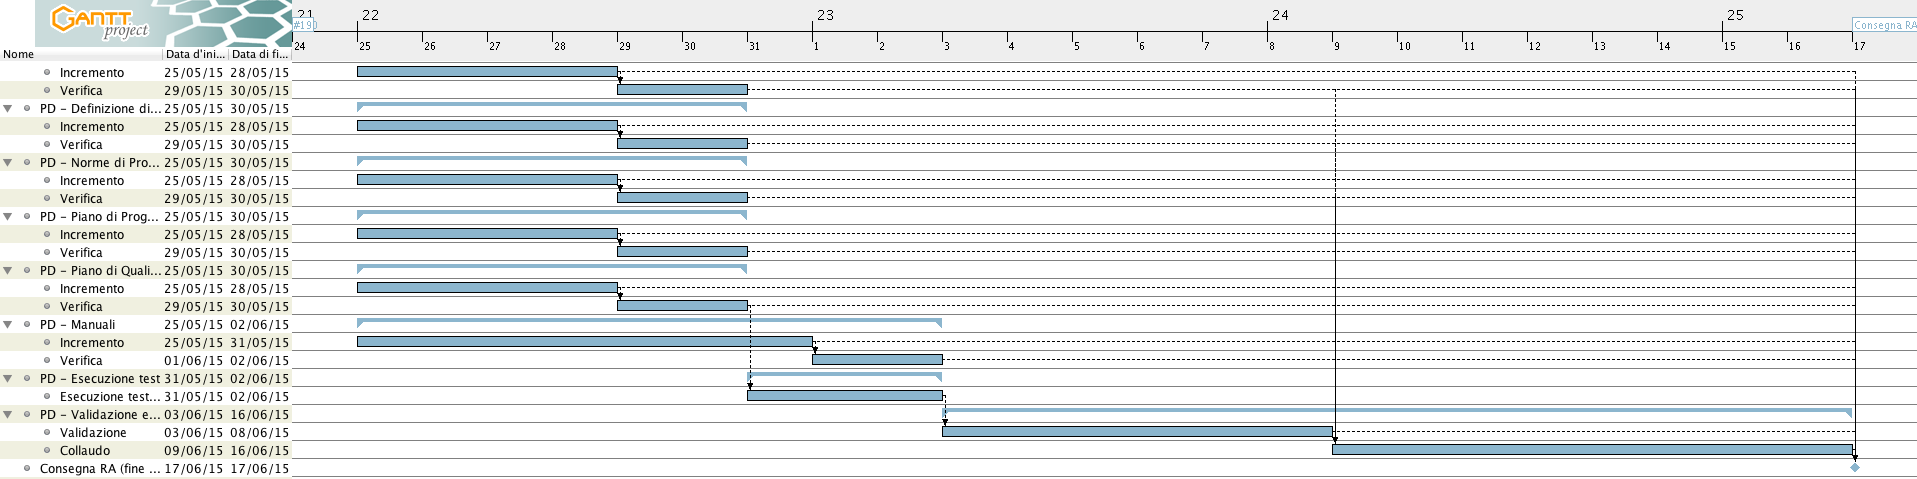
\includegraphics[width=\textwidth]{PianoDiProgetto/Pics/FasePD.png}
		\caption{Gantt Fase PD}
\end{figure}
